Preamble here.

\section{Visualized Performance Metrics}

\section{Structural Overlay Properties}


\section{System Architecture}
\begin{table}[h]
\centering
\resizebox{\columnwidth}{!}{%
\begin{tabular}{ll}
\toprule
Method Name                                       & Returns\\
\midrule
\tt long reportId()                      & The unique id of this node\\
\tt long[] reportNeighborIds()           & The unique ids of this node's neighbors\\
\tt long[] reportTopics()                & List of topic ids this node subscribes to\\
\tt long reportControlMsgsReceived()     & Number of overlay control messages received\\
\tt long reportControlMsgsSent()         & Number of overlay control messages sent\\
\tt long reportControlBytesReceived()    & Number of overlay control bytes received\\
\tt long reportControlBytesSent()        & Number of overlay control bytes sent\\
\tt PubMessage[] reportPubMsgsReceived() & Reports list of publication messages received\\
\tt PubMessage[] reportPubMsgsSent()     & Reports list of publication messages was sent\\

% \emph{reportDuplicatePubMessages(int topic, int messageId)} :  The number of duplicates received for a specific publication\\
% \hline
\end{tabular}
}%
\caption{Reporter Interface Methods}
\label{table:interface}
\end{table}



% ../tables/pubmessage.tex
\begin{table}[]
\centering
\resizebox{\columnwidth}{!}{%
\begin{tabular}{ll}
\toprule
Message item           & Description\\
\midrule
\tt long  MsgId            & Unique id of the this message\\
\tt long  TopicId          & Topic id for which this message was generated\\
\tt long  SourceId         & Id of the previous hop node\\
\tt long  DestinationIds[]   & Ids of the next hop nodes\\
\tt long  OriginalSenderId & Node id of the message source\\
\tt long  TimeStamp        & Timestamp of the message sent/received\\
\end{tabular}
}%
\caption{Data Structure of a Publication Message}
\label{table:structure}
\end{table}



\begin{figure}
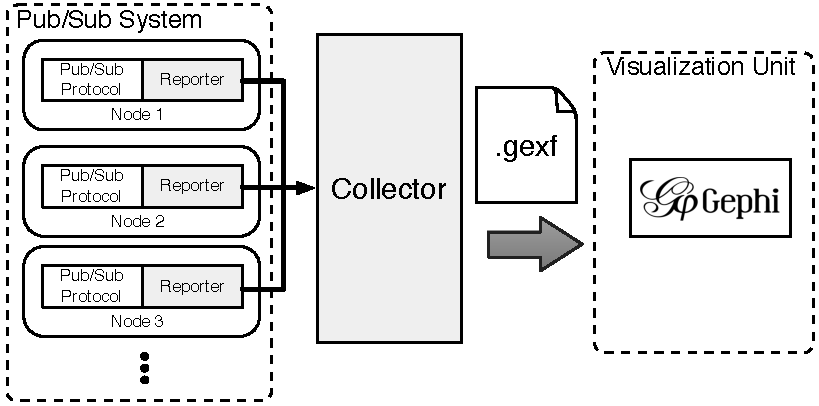
\includegraphics[width=\linewidth]{figures/arch}
\caption{Architecture diagram of \demo}
\label{fig:arch}
\end{figure}
\section{Examples of visualizations for PolderCast and Scribe}
\section{VizPub as a tool for evaluating pub/sub systems }
\subsection{Benefits to our approach}

\section{Using Test-Driven Development}

Software Development Methodology is an active area of research
which is in part driven by the business needs of the private
sector\cite{janzen2005test}. One popular practice is so-called Test-Driven
Development (TDD). The promoters of TDD claims it increases
productivity and reduces the number of bugs and defects in the
code significantly~\cite{beck2003test}. Research
efforts performed at IBM~\cite{maximilien2003assessing} seems to
lend credibility to these claims. However, the use of TDD is not
prevalent in academia, and in~\cite{janzen2005test} they
recommend further research into the field in order to better
determine its effects.

Using TDD means writing tests before writing any code. There are
different types of test. \emph{Unit Tests} targets small,
independent pieces of code, typically methods within a single
module or component, while \emph{Integration Tests} aim to test
code across such modules and components in order to determine
how well they integrate with each other. In our work, we only
took advantage of Unit Tests where suitable using the
JUnit~\cite{junit} and Mockito~\cite{mockito} libraries.
We could also have benefited from a suite of integration tests,
as our implementation is heavily dependent on interoperating
components, as well as file and network IO\@. However, writing
these sort of tests would simply be too time consuming compared
to writing smaller unit tests.

The TDD approach to software development is best described through the
Red-Green-Refactor mantra, which is a central part of the
TDD-philosophy. It can be described through the following steps:

\begin{description}
    \item[Step 1:] Write a test that fails. (Red)
    \item[Step 2:] Make the test pass. (Green)
    \item[Step 3:] Refactor the code while making sure the test
        still passes. (Refactor)
\end{description}

In our experience this routine has been helpful when working
with our implementation code, as it enables us as developer to
refactor with confidence achieving more maintainable code and a
more thoughtful software design. Since we share our
implementation code with the research community by hosting it in
a open repository, any tool or method that helps us improve the
design and maintainability of our project is of great value to
us. Using TDD forced us to think more deeply about what
functionality to implement and how to structure and split the
problem domain into smaller function points. We believe that in
the end, following TDD where its suitable is beneficial to both
programmer productivity as well as programmer happiness. Also,
we are confident that this practice decreased the amount of
technical debt in our project, a problem we find to be commonplace in academia.

/section{Examples of visulizations}
/subsection{Subscription size}
